\documentclass[a4paper, oneside, DIV = 12, 12pt, headings = normal]{scrartcl}


%%% Support for color
\usepackage{xcolor}
\definecolor{lightblue}{HTML}{03A9F4}
\definecolor{red}{HTML}{F44336}
%%%

%%% Graphics inclusion
\usepackage{graphicx}
%%%

%%% Font selection
\usepackage{fontspec}

\setromanfont{STIX Two Text}[
	SmallCapsFeatures = {LetterSpace = 5},
]

\setsansfont{Source Sans Pro}[
]

\setmonofont{Source Code Pro}[
]
%%%

%%% Math settings
\usepackage{amsmath,unicode-math}
\setmathfont{STIX Two Math}

% \usepackage{IEEEtrantools}
\usepackage{mleftright}
%%%

%%% Font settings for different KOMA Script elements
\setkomafont{pagenumber}{\rmfamily}
\setkomafont{disposition}{\rmfamily\bfseries}
%%%

%%% Typographic enhancements
\usepackage{microtype}
%%%

%%% Language-specific settings
\usepackage{polyglossia}
\setmainlanguage{ukrainian}
%%%

%%% List settings
\usepackage{enumitem}
\setlist[enumerate]{
	leftmargin = *,
}
%%%

%%% Captions
\usepackage{caption}
\usepackage{subcaption}

\DeclareCaptionLabelFormat{closing}{#2)}
\captionsetup[subtable]{labelformat = closing}
\captionsetup[subfigure]{labelformat = closing, position = auto}
%%%

%%% Links and hyperreferences
\usepackage{hyperref}
\hypersetup{
	colorlinks      = false,
	linkbordercolor = red,
	urlbordercolor  = lightblue,
	pdfborderstyle  = {/S/U/W 1.5},
}
%%%

%%% All caps
\newcommand{\allcaps}[1]{{\addfontfeatures{LetterSpace = 3}#1}}
%%%

%%% Ceiling function typesetting
\newcommand{\ceil}[1]{\mleft\lceil#1\mright\rceil}
%%%

\begin{document}
	\begin{titlepage}
	\centering
		Міністерство освіти і науки України\\
		Національний авіаційний університет\\
		Навчально-науковий інститут комп'ютерних інформаційних технологій\\
		Кафедра комп'ютеризованих систем управління

		\vspace*{\fill}

		Лабораторна робота №5\\
		з дисципліни «Архітектура комп'ютерів»\\
		на тему «Динамічна пам'ять з довільною вибіркою»\\
		% Варіант №4

		\vspace*{\fill}
		
		\begin{flushright}
			Виконав:\\
			студент ННІКІТ СП-225\\
			Клокун В.\,Д.\\
			Перевірив:\\
			Зіньков Ю.\,Г.
		\end{flushright}

		Київ 2018
    \end{titlepage}

		\section{Мета роботи}
			Оволодіти знаннями та практичними навичками з проектування динамічної пам'\-яті з довільною вибіркою.
			
		\section{Хід роботи}
			Для створення динамічної пам'\-яті з довільною вибіркою необхідно розглянути відповідну схему роботи~(рис.~\ref{fig:memory-working-principle-schematic}). Проаналізувавши її, зможемо побудувати необхідну електронну схему. При побудові необхідно дотримуватись таких правил:
			\begin{enumerate}
				\item На структурній схемі зображують усі основні функціональні частини виробу (елементи, пристрої та функціональні групи) та основні взаємозв'язки між ними. 
				\item Функціональні частини на схемі зображують у вигляді прямокутників чи умовно-графічних позначень.
				\item Графічна побудова схеми повинна надавати найкраще представлення про послідовність взаємодії функціональних частин виробу.
				\item На лініях взаємозв'язків рекомендується позначати стрілками напрям ходу процесів, що протікають у виробі.
				\item На схемі повинні бути вказані найменування кожної функціональної частини виробу, якщо для її позначення був використаний прямокутник.
				\item На схемі дозволяється зазначати тип елемента (пристрою) і/або позначення документа, на основі якого цей елемент (пристрій) використаний.
				\item При зображенні функціональних частин у вигляді прямокутників найменування, типи й позначення рекомендується вписувати всередину прямокутників.
				% \item У випадку великої кількості функціональних частин дозволяється замість найменувань, типів та позначень вказувати порядкові номери справа від зображення або над ним, як правило, згори донизу та зліва направо. У такому випадку найменування, типи та позначення вказують у таблиці, що наводиться на полі схеми.
			\end{enumerate}
			\begin{figure}[!htbp]
				\centering
					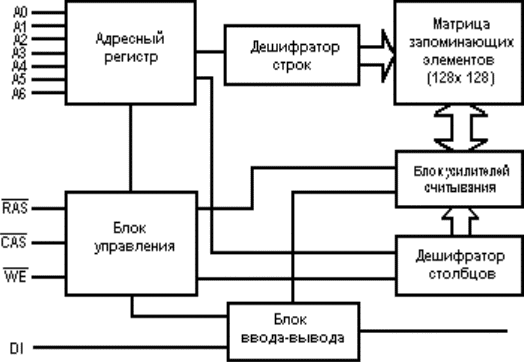
\includegraphics[height = 11\baselineskip]{./assets/01.png}
				\caption{Схема роботи пам'\-яті}
				\label{fig:memory-working-principle-schematic}
			\end{figure}

			При проектуванні ДП з довільною вибіркою треба ознайомитись зі схемою рівнів пам'\-яті~(рис.~\ref{fig:memory-hierarchy}) та схемою пам'\-яті для роботи з великим об'ємом даних~(рис.~\ref{fig:large-data-memory-schematic}).
			% При проектуванні динамічної пам'\-яті з довільною вибіркою треба ознайомитись з рівнями пам'\-яті~(рис.~\ref{fig:memory-hierarchy}).
			\begin{figure}[!htbp]
				\centering
					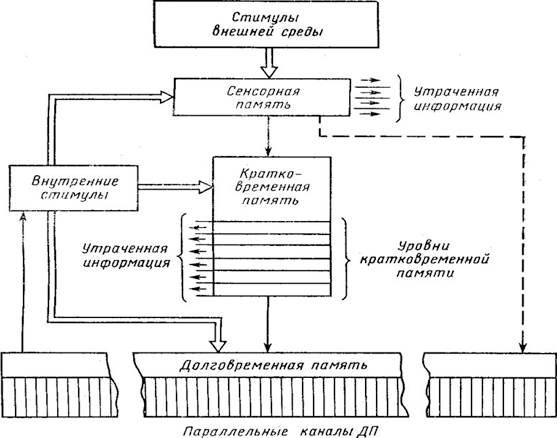
\includegraphics[height = 12\baselineskip]{./assets/03.png}
				\caption{Схема рівнів пам'\-яті (за Г.\,А.\,Вартаняном, М.\,І.\,Лоховим)}
				\label{fig:memory-hierarchy}
			\end{figure}
			\begin{figure}[!htbp]
				\centering
					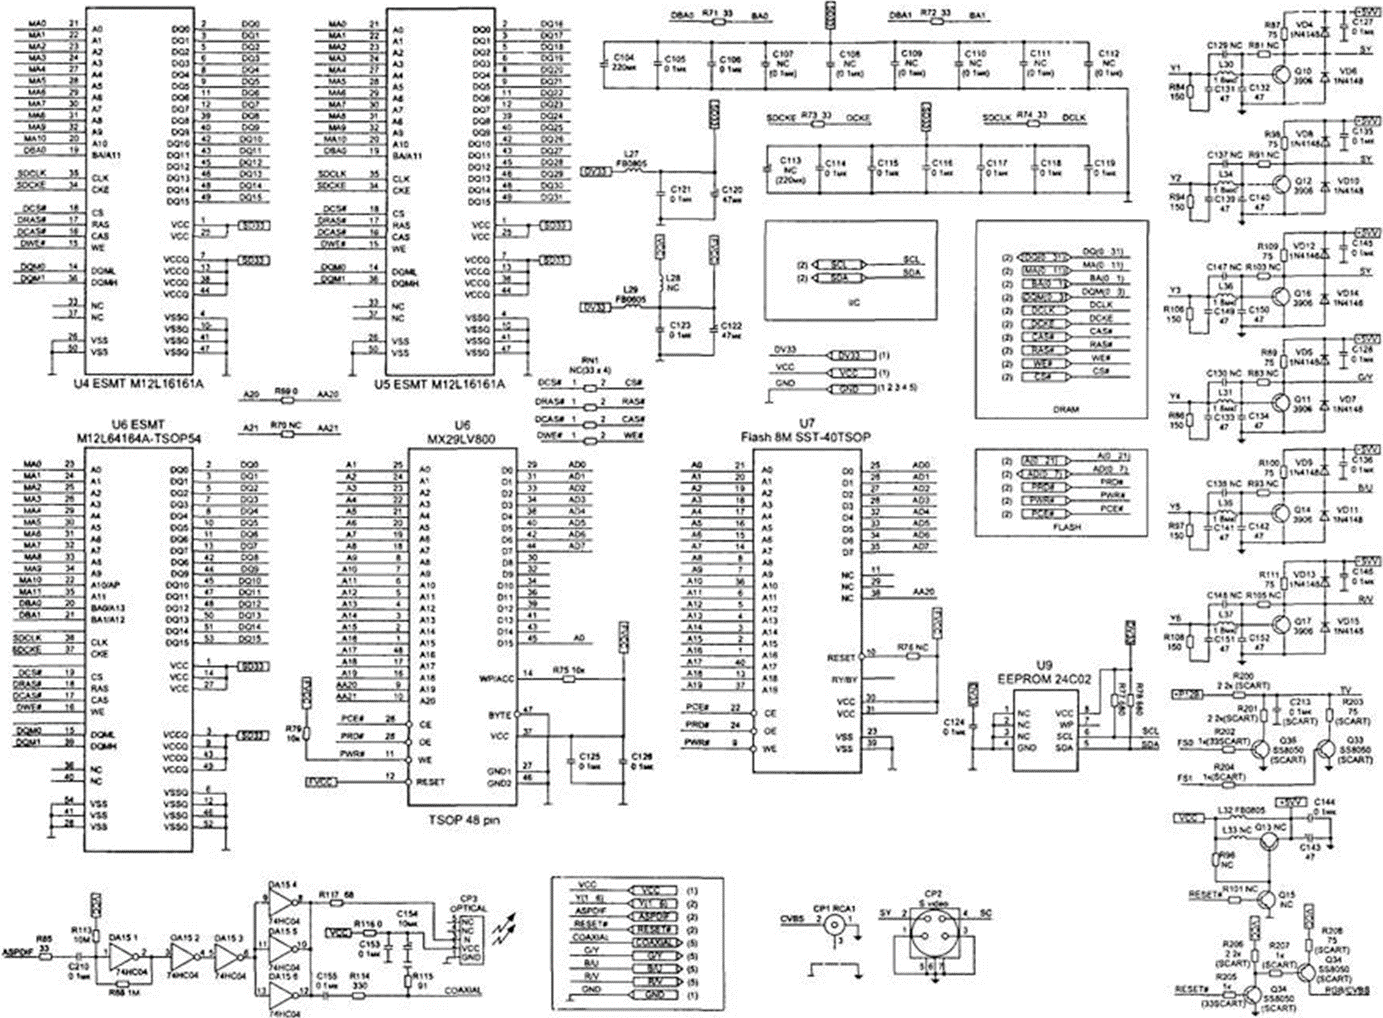
\includegraphics[width = \linewidth]{./assets/04.png}
				\caption{Схема пам'\-яті для роботи з великим об'ємом даних} 
				\label{fig:large-data-memory-schematic}
			\end{figure}

			На основі отриманих даних була побудована електронна схема реалізації динамічної пам'\-яті з довільною вибіркою~(рис.~\ref{fig:memory-schematic-result}).
			\begin{figure}[!htbp]
				\centering
					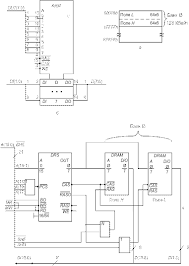
\includegraphics[]{./assets/02.png}
				\caption{Електронна схема реалізації пам'\-яті}
				\label{fig:memory-schematic-result}
			\end{figure}

		\section{Висновок}
			Під час виконання даної лабораторної роботи ми оволоділи знаннями та практичними навичками з проектування динамічної пам'\-яті з довільною вибіркою.

\end{document}

